\chapter{State of the art} \label{chap:sota}

\section*{}
In this chapter it is described the current state of the art in Mining Software
Repositories (MSR), by reviewing findings and discussing existing defect
prediction techniques. Related tools are presented and Crowbar, the fault
localization tool that we aimed to improve with the defect prediction results.

\section{Best practices and recommendations}
Hemmati \textit{et al.} analyzed the last decade of mining software
repositories publications, between 2004 and 2012, and produced an article
with best practices and recommendations to new researchers in the MSR
community \cite{Hemmati2013}. The main activities of Mining Software
Repositories research are: data extraction and preparation, synthesis,
analysis and sharing results.

\subsection{Data extraction and preparation}
In data extraction the source code is the most important artifact, although
communication artifacts can be used such as emails and issue trackers like
Bugzilla. The problem in this phase is the use of wrong assumptions since it
is important to understand how the Control Version System is used, the
project and its domain since exists noisy data \cite{herzig-tr-2012}. For
example, a commit message may not reflect the change and can be used only as
a way of communication. Also, the study of developers and their behavior can
produce valuable information, but the problem of multiple online personas
representing the same person should be considered.

\subsection{Synthesis}
Synthesis is the phase that involves the prediction and machine learning
algorithms that are feed from the extracted data. If we are doing regression
analysis, that is estimating the relationship of variables, it is important to
be aware of the assumptions used.

\subsection{Analysis}
Results of the synthesis phase are analyzed and interpreted, being considered
the most important part of MSR research. A manual inspection of the analysis
outputs is required because the use of heuristics and automation may be
inaccurate. Since may not be feasible analyzing everything, developers can use
just sample data. If prediction or classifiers are used in the synthesis phase,
the effectiveness is enough to evaluate the results (recall and recognition).

\subsection{Sharing results}
In MSR sharing results is usually ignored because most of research is based on
empirical studies and do not share data. It is suggested that the raw and
processed data should be shared along with the tools used, to push the community
forward. In 2005 the number of published papers in MSR was 9 and in 2012 was
44 \cite{Hemmati2013}. The themes with most publications are data extraction
and modeling.


\section{Research on Mining Software Repositories}
There is relevant work in MSR research capable of extracting insights about
repositories, such as finding who is the best developer to fix a bug
\cite{Servant1}. This research is also published in the MSRconf
\footnote{\url{http://msrconf.org}}, that is an annual conference that joins
researchers in this area of study.

\subsection{History slicing}
Servant and Jones developed a technique called history slicing that enables
developers to track code evolution at the line of code level, since current
SCMs require a considerable developer effort to analyze code changes at
this granularity \cite{Servant}. This technique provides the minimal amount of
information about the code changes and its implementation is called CHRONOS.
The motivation behind this technique is that, by observation, researchers
concluded that developers ask often about the last code changes and the complete
history to understand why a software component was implemented in a certain way.

\subsection{Identifying types of bugs}
Chadd C. Williams and Jeffrey K. Hollingsworth proposed a technique that
compares code changes and the types of bugs being fixed
\cite{ChaddC.WilliamsandJeffreyK.Hollingsworth2005}. This approach does not
analyze commit messages because it is hard to correlate bug reports and code
changes. The most common types of bugs are analyzed, such as functions that do
not check if a variable is null, and then the list of warnings is ranked to
avoid false positives. Further work is necessary to improve this technique such
as analyzing other types of bugs.

\subsection{Whosefault}
Francisco Servant proposed an approach that helps to find the most suitable
developer to fix a bug and where the bugs are located \cite{Servant1}. The
algorithm to find what is the right developer to fix the bug is called
Whosefault and depends on statistical coverage-based fault-localization
techniques. This algorithm have an accuracy of up to 37\%.

\subsection{Classification of bugs}
Classification of bugs is an important problem in MSR due the presence of noise.
For example, a commit can be described as a fix on the message but can be also
introducing new features. To avoid mixing new features and bug fixes in the
same patch, some standards can be enforced to ensure they are classified the
right way on the issue tracker
\footnote{\url{https://docs.python.org/devguide/patch.html}}.

The estimated impact of misclassification in defect prediction, is flagging
components as defective that do not have any bugs, on an average of 39\%
\cite{herzig-tr-2012}. The quality of diagnosing defective components depends
on the quality of data. Kim Herzig \textit{et al.} found data quality issues,
after investigating the projects HTTPClient, Jackrabbit, Lucene-Java, Rhino
and Tomcat5 \cite{herzig-tr-2012}:

\begin{description}
  \item[Issue reports classifications are unreliable] \hfill \\
  In the issue trackers investigated, at least 40\% of reports are misclassified.
  \item[Every third bug is not a bug] \hfill \\
  33,8\% of bug reports are not bugs.
\end{description}

These researchers also pointed that the main source of wrong reports are
related to the fact that developers and users have different perspectives on bug
classification.

\subsection{Mining Git repositories tools}
Mining a repository is the first step to extract data to feed defect prediction
models. Git repositories usage is growing and are different from SVN
repositories because they are decentralized. The advantage of this
characteristic is that the information extraction is done locally
\cite{Sadowski2011}. Some tools were developed to extract information from Git
but the problem is that they are poorly documented, project specific and there
are no standards about how to share mining results \cite{Carlsson638844}.

There are some existing tools that extract data from Git repositories:

\begin{description}
    \item[git\_mining\_tools] \hfill \\
    It is developed in Ruby, extracts data from a Git repository and exports to
    a PostgreSQL or MySQL database. The source code is available on Github
    \footnote{\url{https://github.com/cabird/git_mining_tools/}}.

    \item[gitdm] \hfill \\
    It is developed in Python and receives the output from the git log command
    and then generates an HTML document with a report. It gathers statistics
    from Linux Kernel patches. The repository of this tool is public
    \footnote{\url{git://git.lwn.net/gitdm.git}}.
\end{description}

\section{Defect prediction techniques}
The estimation of component's reliability helps us evaluate from a set of
components what are the most bug-prone and then focusing the resources to fix
them \footnote{\url{http://www.cse.ust.hk/~hunkim/Research.html}}. Despite the
existing research, organizations still ask how they can evaluate the quality of
their software \cite{815326}.

It is important to note that developers must consider that defect prediction
is not completely accurate and it should be combined with other practices.

\subsection{Approaches}
Defect prediction approaches can be divided into three main categories
\cite{D'Ambros:2012:EDP:2318097.2318149}:


\begin{description}
  \item[Change log] \hfill \\
  It uses metrics from control version systems and use assumptions, such as:
  the files with most changes are must bug-prone;
  \item[Single-version] \hfill \\
  It analyzes the current state and behavior of the system;
  \item[Effort-aware]  \hfill \\  This approach does not predict if components
  are buggy, but estimates the ones that require more effort to inspect bugs.
\end{description}

The approaches that are most interesting to us, according to our goals of mining
software repositories, are change log approaches. There is a mindmap, that
gives an overview of the different defect prediction approaches that is
published in Mindmeister\footnote{\url{https://www.mindmeister.com/506039387}}.

\subsection{Metrics}
There are metrics to analyze such as Process, Previous defects, Source code and
Entropy of Changes \cite{D'Ambros:2012:EDP:2318097.2318149}.

\begin{description}
  \item[Process] \hfill \\
  Bugs are caused by changes and for each file the metrics can be the number
  of revisions, fixes, authors, refactorings, etc
  \cite{Moser:2008:CAE:1368088.1368114}. The number of revisions and fixes are
  the ones that perform better
  \cite{Zimmermann:2007:PDE:1268984.1269057, 859533}.

 \item[Previous defects] \hfill \\
 Past defects predict future defects. The metrics can be the number of past
 fixes and the categories of bugs, according to a severity scale. Zimmermann et
 al. concluded that there exists a high correlation between previous and future
 defects \cite{Zimmermann:2007:PDE:1268984.1269057}.

 \item[Source code] \hfill \\
 Complexity of components is correlated with the effort of changing them. The
 metrics used are lines of code, object oriented metrics (e.g. number of
 attributes) and Chidamber \& Kemerer metrics (e.g. Lack of cohesion in methods)
 \cite{295895}.

 \item[Entropy of changes] \hfill \\
 Complex changes are usually more bug-prone. For example, a commit that changes
 only one file is simpler that one that changes multiple files.
\end{description}

A study concluded that for flagging components that are buggy (binary
classification), process metrics perform better but, for ranking components,
source code metrics are better suited \cite{D'Ambros:2012:EDP:2318097.2318149}.

\subsection{Time-Weighted Risk}
A technique used at Google is Time-Weighted-Risk (TWR). It is a simple way of
estimating component's reliability, easy to understand and a result of a case
study \cite{Chris2013}. In this model, components are files and those files
have commits in certain timestamps. Therefore, for each component a score is
computed and those that have the highest score are less reliable so they might
have more bugs. The formula is the following:

\begin{equation}
 Score = \sum_{ i=0}^{n} \frac{1}{1 + \mathrm{e}^{-12ti + 12}}
\end{equation}

The score is a sum of all the bug-fixing commits given their normalized
timestamps \( ti\), from 0 to 1 where 0 is the start of the repository and 1 it
is the last committed time. This model gives more importance to the most recent
changes because it uses time to compute the score, so it is able to distinguish
components with the same number of fixes if they were fixed in different
timestamps. The curve of TWR function \ref{eq:twr_function} is described in
figure \ref{figure:twr_graph}.

\begin{equation}
\label{eq:twr_function}
twr(t_i) = \frac{1}{1 + e^{-12t_i + 12}}
\end{equation}

\begin{figure}[H]
    \begin{center}
        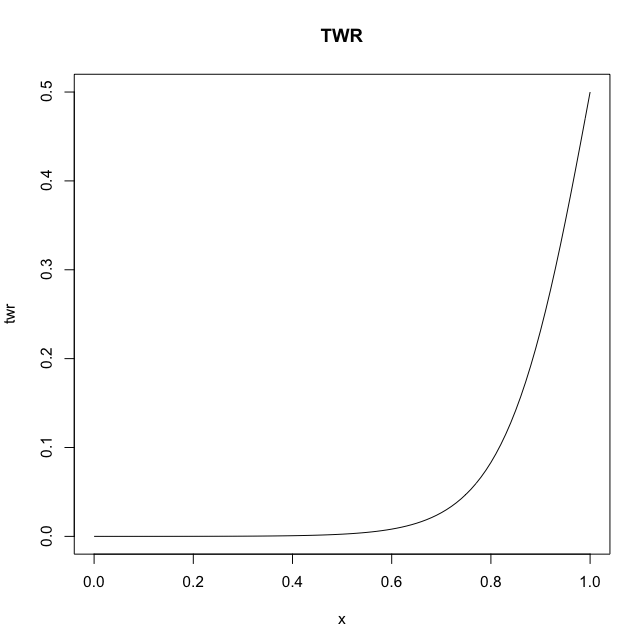
\includegraphics[scale=0.5]{twr_graph}
        \caption{Time Weighted Risk (TWR)}
        \label{figure:twr_graph}
    \end{center}
\end{figure}

\subsubsection{Example}
Given the repository represented in tables \ref{table:repo_files_commits} and
\ref{table:repo_commits}:

\begin{table}[H]
    \caption{Repository example -  files and commits}
    \label{table:repo_files_commits}
    \begin{center}
        \begin{tabular}{ | l | l | l | }
            \hline
            File & Commits \\ \hline
            main.java & A,B,C \\ \hline
            gui.java & A,D\\ \hline
            core.java & A  \\
            \hline
        \end{tabular}
    \end{center}
\end{table}

\begin{table}[H]
    \begin{center}
        \caption{Repository example - commits}
        \label{table:repo_commits}
        \begin{tabular}{ | l | l | l | }
            \hline
            Commit & Time & Bug fix? \\ \hline
            A & 5 & no \\ \hline
            B & 10 & no\\ \hline
            C & 15 & yes  \\ \hline
            D & 30 & yes  \\ \hline
        \end{tabular}
    \end{center}
\end{table}
Considering the current timestamp is 50 and the one of the beginning of the
repository is 5, the normalized timestamp for the bug-fixing commits are the
following:

\begin{equation}
ti_C = \frac{15 - 5}{50 - 5} = \frac{2}{9}\qquad
ti_D = \frac{30 - 5}{50 - 5} = \frac{5}{9}
\end{equation}

Using the previous timestamps, the scores for each file are:

\begin{equation}
Score_{main} \approx 0.000088 \qquad
Score_{gui} \approx 0.004805 \qquad
Score_{core} = 0
\end{equation}

Considering this model, the less reliable component is gui.java because it has
the highest score due the fact that exists a recent bug-fixing commit. If
someone asked you to find bugs in a repository you would do the same: inspecting
the files with the most commits related to bugs.

\subsubsection{Discussion}
TWR gives more importance to the most recent changes and that is a way of not
flagging old untouched files that developers do not want to fix. But, the
model is not complete enough because files that have score equal to zero may
have unfixed bugs. Therefore, these model should be improved with information
from others techniques.

Research has been done at Google where developers had the opportunity to choose
between this model and Fixcache (further discussed) and by seeing the results of
both of the algorithms, developers chose TWR, mainly because it considers the
most recent changes \cite{Chris2013}. The study revealed developers are
\"afraid\" of old source code so a model that highlights those old components
cannot be considered good.

\subsection{Fixcache and Bugcache}
Fixcache and Bugcache are defect prediction models based on cache and the
difference from other models is that they are more dynamic and have more
predictive power \cite{Kim:2007:PFC:1248820.1248881}. This models assume that
faults do not occur in isolation but in burst with other related faults.

A cache is a list of components where the granularity can be the executable
binary, module, file or method (entity). Since faults appear in bursts, the
cache is updated by the following policies:

\begin{itemize}
  \item new or modified files may have bugs (new and changed locality);
  \item buggy files can contain more bugs (temporal locality);
  \item files changed with buggy files may have bugs (spacial locality).
\end{itemize}

The size of the cache is fixed and when it is full, a policy of removal should
be chosen: the component to remove can be the least recent used (LRU), number
of recent changes, number of recent bugs and the number of authors. LRU is the
policy that performs better \cite{Sadowski2011}.

Fixcache updates the cache when the bug is fixed and Bugcache when the bug is
introduced. The bug-fixing changes are detected by mining the repository commits
and bugs database. Bug-introducing changes are detected by the bug-fixing
changes. For example, if file A has been fixed in a certain commit, the commit
that created this file is a bug-introducing change. Due the presence of false
positives, this technique can be improved by using bug databases.

A study concluded that Fixcache not only can do bug prediction in a certain
point of time but can predict with accuracy at weekly intervals
\cite{Sadowski2011}.

\subsection{Change Classification}
Change Classification model evaluates if a change will introduce a bug using
machine learning techniques by learning from previous bugs~\cite{Kim2008}. A
problem that may arise is the effect of noise in the training set, compromising
the recall and recognition of buggy changes, but techniques are available to
reduce this noise. The classifier decides if a change is buggy or clean with
78\% accuracy and 60\% percent bug recall on average~\cite{Kim2008}. This
technique has less prediction power but knowing that a commit introduced a
bug it is still useful. The main characteristics are:

\begin{itemize}
  \item classify changes at the file level as buggy or clean;
  \item detect when a bug is introduced and not when it is fixed;
  \item takes advantage of source code information (features);
  \item independent of the programming language using bag-of-words methods.
\end{itemize}

Support Vector Machines is the approach used to classify changes due its
performance in text classification applications. Change Classification can be
used as a commit checker, a bug indicator on source code editing and can change
the software engineering process by giving immediate feedback to trigger a code
inspection when a commit is made \cite{Kim2008}.

Some limitations are important to consider such as the process of extracting
features that depends how developers used Git and like other machine learning
approaches, it takes time to learn.

\section{Fault localization techniques}
Fault localization is the process of finding the component causing the software
execution deviating from its expected result. Traditionally, developers use
manual techniques just as injecting prints to debug values or breakpoints.
Automatic fault localization techniques are used to reduce the cost of finding
these faulty components.

\subsection{Program-spectra based}
Program-spectra based methods evaluates the probability of each component being
faulty by analyzing the program execution history \cite{Perez2004}. It is a
statistical technique that, for each test case, computes the spectrum, that is
the code coverage and execution result. The program spectrum is then the list
of test cases execution results and can be easily understood by the example in
table \ref{table:spectrum}.

\begin{table}[H]
    \begin{center}
    \caption{Program spectrum}
    \label{table:spectrum}
    \begin{tabular}{ | c | c | c | c | c | c |}
        \hline
        Test Case & Component A & Component B & Component C & Result \\ \hline
        T1 & X & & & Success \\ \hline
        T2 & X & X & & Failure \\ \hline
        T3 &  & X & & Failure \\ \hline
        T4 & X &  & X & Success \\ \hline
    \end{tabular}
    \end{center}
\end{table}

To determine what components are called in each test case it is used code
instrumentation. The program spectrum in table \ref{table:spectrum} use binary
flags so it is called hit spectra. From this input, the components that most
affects program execution are computed, calculating similarity coefficients
using the Ochiai formula \cite{Abreu:2009:SMF:1747491.1747511}. This technique
also exploits information from execution outcomes. The output is then the
similarity coefficient for each component, that is their likelihood of
containing the fault.

Spectrum Fault Localization (SFL) approaches have a good quality of diagnosis
and scale well, but is more accurate when the system have many test cases
\cite{Mayer2008}. There are some tools based on SFL such as:

\begin{description}
  \item[Gzoltar] \hfill \\
  An eclipse plugin\footnote{\url{http://gzoltar.com/}} that integrates with
  JUnit tests \cite{Campos:2012:GEP:2351676.2351752}.
  \item[Tarantula] \hfill \\
  A technique and a tool\footnote{\url{http://spideruci.org/fault-localization/}}
  that offers recommendations to reduce the time needed to find the fault
  \cite{jones05}.
\end{description}

\subsection{Model-based}
Model-based techniques use reasoning to do fault localization by having the
system knowledge a priori. The system model, the description of correct
behavior, is used to compare with the observed behavior of the program and then
the difference is used to identify components that explain this deviation
\cite{Mayer2008}. Since model-based approaches in software engineering require a
formal specification, to avoid this limitation the model is obtained by
inference from test cases \cite{Perez2004}. The type of model can be:

\begin{itemize}
  \item based on dependencies between program statements;
  \item based on computing values propagation;
  \item based on creating abstraction models for particular fault assumptions.
\end{itemize}

Model-based fault localization should be combined with others techniques since
the current approaches are not efficient, with high computational cost and scale
poorly.

\subsection{Barinel}
Barinel is a combination of Spectrum-based fault localization and Model Based
Diagnostic \cite{Abreu:2009:SMF:1747491.1747511}. It starts by receiving a
hit-spectra matrix, that contains the observation of running the test cases.

\newcommand{\pr}{\mbox{Pr}}
\newcommand{\likelihood}{\pr(obs_i, e_i \mid d)}
\newcommand{\gFunc}[1][d]{\displaystyle\prod_{j \in (d \cap obs_i)} g_j}

\begin{figure}[h]
  \begin{center}
    \begin{tabular}{c|ccc|c}
    	& \multicolumn{3}{|c|}{$obs$} &      \\
      & $c_1$ & $c_2$ & $c_3$ & e     \\ \hline
      $t_1$ & 1     & 1     & 0     & 1     \\
      $t_2$ & 0     & 1     & 1     & 1     \\
      $t_3$ & 1     & 0     & 0     & 1     \\
      $t_4$ & 1     & 0     & 1     & 0     \\
    \end{tabular}
  \end{center}
  \caption{Hit-spectra matrix example}
  \label{figure:hit_spectra}
\end{figure}

Figure \ref{figure:hit_spectra} shows an example of a hit-spectra matrix, with
the outcome $e$ of every test case $t$ and the components involved. For example,
test case $t_1$ hits components $\{c_1, c_2\}$ and fails.

The algorithm then takes the following steps:
\begin{description}

\item[Candidate generation] \hfill \\
Only minimal candidates are generated. A candidate \( d \) is a set of
components that explains the observed behaviour of the program. In this example,
the list of candidates are:
\begin{itemize}
\item \( d_1 = \{c_1, c_2\} \)
\item \( d_2 = \{c_1, c_3\} \)
\end{itemize}

\item[Candidate ranking] \hfill \\
Each candidate \( d \)  is evaluated by computing the posterior probability
using the Na\"ive Bayes rule:

\begin{equation}
	\pr(d\mid obs,e) =  \pr(d) \cdot \prod_{i}\frac{\likelihood}{\pr(obs_i)}
\end{equation}

The denominator $\pr(obs_i)$ is a term that is normalized for all candidates
and it is not used for ranking. Let \( p_j\) denote the prior probability of a
component being faulty. Then, the prior  $\pr(d)$  of a candidate $d$ is:

\begin{equation}
  \pr(d) = \prod_{j \in d} p_j \cdot \prod_{j \notin d} (1 - p_j)
\end{equation}

Let $g_j$ denote the probability of a component behaving normally (goodness).
Then $\pr(obs_i,e_i \mid d)$ is computed by:

\begin{equation}\label{eq:likelihood_func}
  \pr(obs_i, e_i \mid  d) =
  \begin{cases}
    \gFunc     & \textrm{if   } e_i = 0 \\
	1 - \gFunc & \textrm{otherwise}
  \end{cases}
\end{equation}

If for a certain component $g_j$ is not available, it is computed by maximizing
$\pr(obs,e \mid d)$ (Maximum Likelihood Estimation (MLE)), for the Na\"ive Bayes
classifier. Considering our example, the probabilities for both candidates $d_1$
and $d_2$ are:

\begin{equation}
    \pr(d_1 \mid obs,e) =
    \overbrace{\bigg(\frac{1}{1000} \cdot \frac{1}{1000} \cdot \bigg(1 - \frac{1}{1000}\bigg)\bigg)}^{\pr(d)}
    \times
    \overbrace{
      \underbrace{(1-g_1 \cdot g_2)}_{t_1}
      \times
      \underbrace{(1-g_2)}_{t_2}
      \times
      \underbrace{(1-g_1)}_{t_3}
      \times
      \underbrace{g_1}_{t_4}
    }^{\pr(obs,e \mid d)}
\end{equation}
%
\begin{equation}
    \pr(d_2 \mid obs,e) =
    \overbrace{\bigg(\frac{1}{1000} \cdot \frac{1}{1000} \cdot \bigg(1 - \frac{1}{1000}\bigg)\bigg)}^{\pr(d)}
    \times
    \overbrace{
      \underbrace{(1-g_1)}_{t_1}
      \times
      \underbrace{(1-g_3)}_{t_2}
      \times
      \underbrace{(1-g_1)}_{t_3}
      \times
      \underbrace{g_1 \cdot g_3}_{t_4}
    }^{\pr(obs,e \mid d)}
\end{equation}
\end{description}

By performing MLE for both functions:
\begin{itemize}
\item $\pr(d_1 \mid obs,e)$ is maximized for $g_1=0.47$ and $g_2=0.19$;
\item $\pr(d_2 \mid obs,e)$ is maximized for $g_1=0.41$ and $g_3=0.50$.
\end{itemize}

Applying the computed values for goodness, $\pr(d_1 \mid obs,e)=1.9 \times
10^{-9}$ and $\pr(d_2 \mid obs,e)=4.0 \times 10^{-10}$. The ranking is then
$(d_1,d_2)$.


\subsection{Crowbar}
Crowbar\footnote{\url{https://crowbar.io}}, formerly known as Gzoltar, is a tool
for Java projects that relies on test cases (dynamic analysis) to help
developers locate where is the fault of a bug. It uses the Barinel algorithm,
combining Spectrum-Based Fault Localization and Model-Based approaches. It
supports granularity until the statement level and use code instrumentation by
injecting probes in the source code.

\begin{figure}[H]
    \begin{center}
        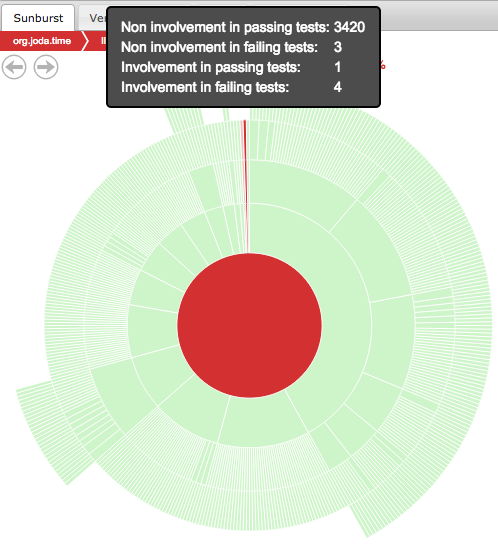
\includegraphics[scale=0.5]{crowbar}
        \caption{Crowbar sunburst chart report}
        \label{figure:crowbar_report}
    \end{center}
\end{figure}

Figure \ref{figure:crowbar_report} shows an example of a sunburst report that
can be zoomed. In this type of visualization, the granularity of components
increases from the center to the exterior (statement) and the colors are a clue
to find faulty components. We also have the possibility to visualize the report
as a vertical partition.

\subsubsection*{Usage}
Crowbar supports Junit\footnote{\url{http://junit.org/}} and
TestNG\footnote{\url{http://testng.org/}}. It runs as a Java agent on the test
suite through the Maven\footnote{\url{https://maven.apache.org/}} Surefire
Plugin\footnote{\url{https://maven.apache.org/surefire/maven-surefire-plugin/}}.
Configuration is done in the file pom.xml\footnote{\url{https://maven.apache.org/guides/introduction/introduction-to-the-pom.html}},
that contains information for Maven about the project and configuration details
to build and test.

Crowbar will then display the results on a web server by displaying an URL that
we must access on a browser to be able to see the report.

\section{Similar tools}
There are plenty of tools available that analyse Software projects. They
evaluate code quality and warn developers about problems detected.

\subsection{Codacy}

Codacy \footnote{\url{https://codacy.com}} is an automatic software revision
service (static analysis) that uses defect prediction models to estimate
software component reliability. It is a Startup based in Lisbon that won the
best pitch award in 2014 Web Summit in London and it is available with free
(Open Source) and paid plans.

This service uses the Change Classification principle, classifying a commit as
buggy or clean. It supports Scala, Javascript, Python, PHP and CSS. With a few
steps it is possible connecting our repository, hosted at Bitbucket or Github.

\begin{figure}[H]
    \begin{center}
        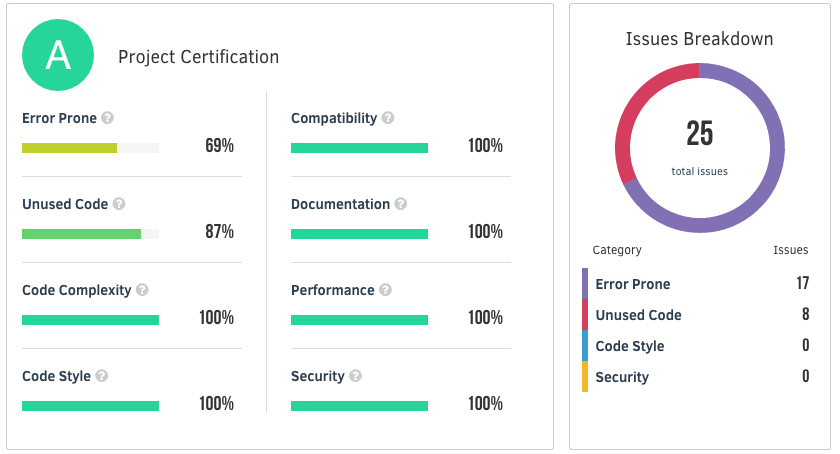
\includegraphics[width=\textwidth]{codacy-report}
        \caption{Codacy dashboard}
        \label{figure:codacy_dashboard}
    \end{center}
\end{figure}

Figure \ref{figure:codacy_dashboard} shows the dashboard with a variety of
metrics, reporting a score for code style, errors, code complexity, performance,
unused code, compatibility, etc. New and fixed issues are presented, therefore,
developers feel rewarded and motivated to improve code quality, a feature that
somehow failed in the tool developed in a research conducted at Google in 2013
by Chris Lewis et al. \cite{Chris2013}.

\subsection{Moskito}
Moskito\footnote{\url{http://moskito.org}} is a tool that monitors Java Web
applications, does fault localization and it is free and Open Source~\footnote{\url{https://github.com/anotheria/moskito-control}}.
Developers must use annotations to declare what classes or methods to monitor
and it does not require changing code, which make this solution simple to use.
Two main elements of this tool are the agent and server, where the first
collects data and sends it to the server, that processes and displays
information in a dashboard.

\begin{lstlisting}[language=java, caption=Usage example from Moskito documentation]
//simply add @Monitor
@Monitor
public class MonitoredClass {
    public void firstMethod(){
        //do something
    }
    public void secondMethod(){
        //do something else
    }
    //you can also exclude methods from monitoring:
    @DontMonitor
    public void doNotMonitorMe(){
    }
}
\end{lstlisting}

\begin{figure}[H]
    \begin{center}
        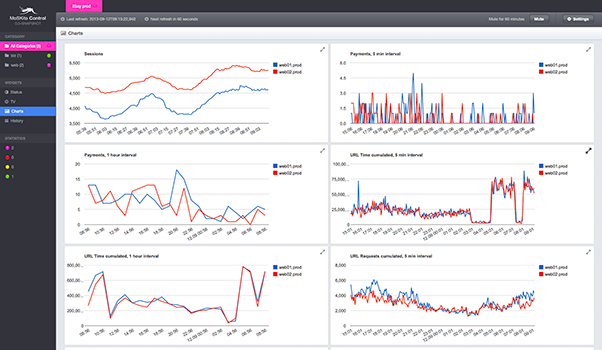
\includegraphics[scale=0.5]{moskito-control}
        \caption{Moskito dashboard}
        \label{figure:moskito_dashboard}
    \end{center}
\end{figure}

The dashboard at figure \ref{figure:moskito_dashboard} displays performance
charts taken from multiple nodes. When a component performance changes, the
health indicator change its color, so developers can fix the problem
immediately, before affecting the whole application and users complain.

\subsection{SensioLabsInsight}
SensioLabsInsight in figure \ref{figure:sensiolabsinsight}, is a web service
\footnote{\url{https://insight.sensiolabs.com/}} that continuously analyzes PHP
projects in terms of security, bugs and other quality checks. It also does
dynamic analysis to improve diagnostic accuracy. Integrates with Github and
Bitbucket services and is free for Open Source projects.

\begin{figure}[H]
    \begin{center}
        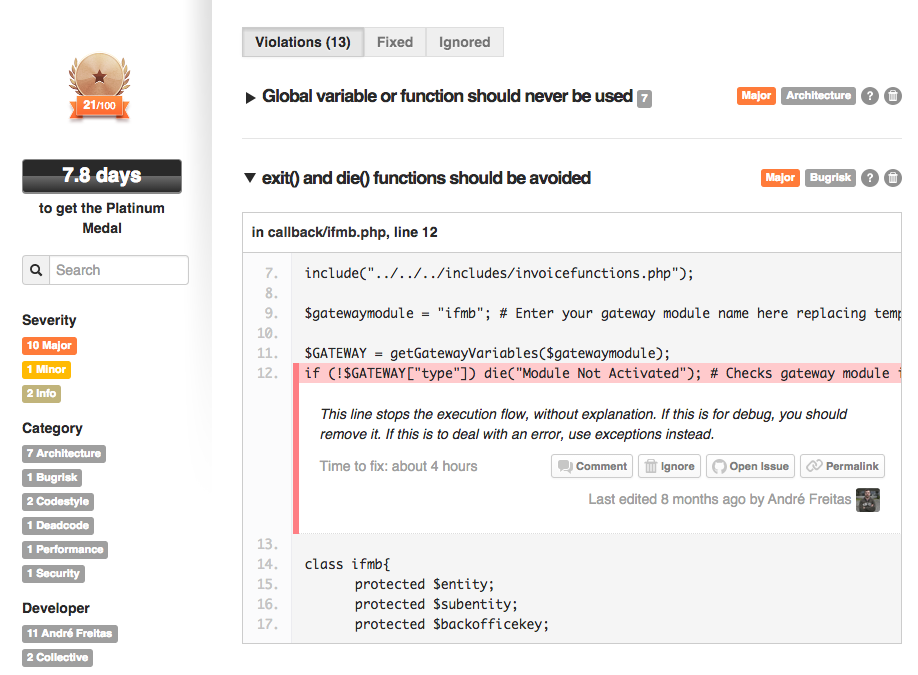
\includegraphics[scale=0.4]{sensiolabsinsight}
        \caption{Example of a report from SensioLabsInsight}
        \label{figure:sensiolabsinsight}
    \end{center}
\end{figure}

\subsection{Code Climate}
Code Climate \footnote{\url{https://codeclimate.com/}} in figure
\ref{figure:codeclimate}, is another service that analyzes PHP, Python,
Javascript and Ruby using static analysis. It essentially produce warnings about
issues in code complexity, duplication, style and readability. Also displays
insights about churn (lines changed) versus code quality. The dashboard is very
complete since we can check listed issues or inspect code along with the
warnings produced. It has a free plan for Open Source projects.

\begin{figure}[H]
    \begin{center}
        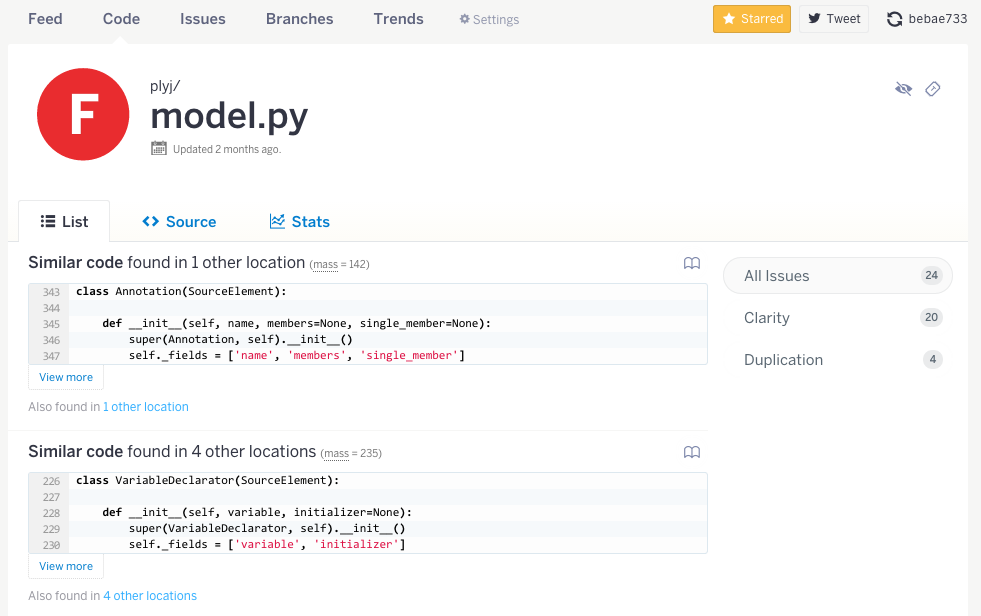
\includegraphics[scale=0.4]{codeclimate}
        \caption{Issues listed on Code Climate}
        \label{figure:codeclimate}
    \end{center}
\end{figure}

\subsection{Pull Review}
Pull Review \footnote{\url{https://pullreview.com/}} in figure
\ref{figure:pullreview}, is an automatic code review service (static analysis)
just for Ruby. It gives feedback for style, duplication, code smells,
documentation, security and tests. It has the ability of linking a Github,
Gitlab or Bitbucket repository and is also free for Open Source.

\begin{figure}[H]
    \begin{center}
        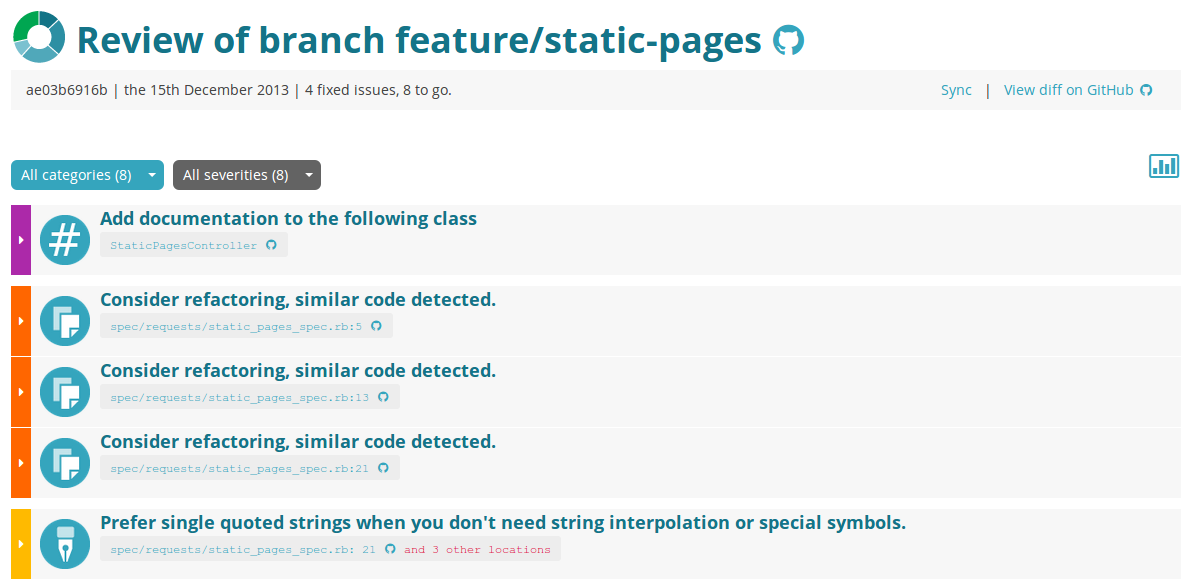
\includegraphics[scale=0.3]{pullreview}
        \caption{Pull Review report}
        \label{figure:pullreview}
    \end{center}
\end{figure}
